\chapter{ทฤษฎีที่เกี่ยวข้อง}
บทนี้จะเป็นรายละเอียดเกี่ยวกับทฤษฎีและงานวิจัยที่เกี่ยวของกับการพัฒนาแอปพลิเคชันในครั้งนี้ โดยแบ่งเนือหาออกเป็น ส่วนได้แก่ ส่วนที่ 1 เครื่องมือที่ใช้ในการพัฒนาแอปพลิเคชัน หัวข้อที่ (2.1) ส่วนที่ 2 ความรู้ภาษาที่ใช้ในการพัฒนาระบบ หัวข้อที่ (2.2-2.3) 
ส่วนที่ 3 ความรู้ของ Library ที่มช้พัฒนาแอปพลิเคชัน หัวข้อที่ (2.4-2.6) ส่วนที่ 4 ความรู้ฐานข้อมูลที่ใช้พัฒนาแอปพลิเคชัน หัวข้อที่ (2.7) 
% \begin{enumerate}[label=2.\arabic*]
% 	\item ความรู้พื้นฐานระบบปฏิบัติการแอนดรอยด์
% 	\item ความรู้พื้นฐานภาษา Java
% 	\item ความรู้พื้นฐานภาษา Python
% 	\item ความรู้พื้นฐาน Tensorflow Lite
% 	\item ความรู้พื้นฐานของระบบ XX เดิม
% 	\item เอกสารและงานวิจัยที่เกี่ยวข้อง
% \end{enumerate}

\section{ความรู้พื้นฐานระบบปฏิบัติการแอนดรอยด์}
	แอนดรอยด์ \cite{bib1} แอนดรอยด์ (Android) คือระบบปฏิบัติการแบบเปิดเผยซอร์ฟแวร์ต้นฉบับ (Open Source) โดยบริษัท กูเกิ้ล (Google Inc.) ที่ได้รับความนิยมเป็นอย่างสูง เนื่องจากอุปกรณ์ที่ใช้ระบบปฏิบัติการแอนดรอยด์ มีจำนวนมาก อุปกรณ์มีหลากหลายระดับ หลายราคา รวมทั้งสามารถทำงานบนอุปกรณ์ที่มีขนาดหน้าจอ และความละเอียดแตกต่างกันได้ ทำให้ผู้บริโภคสามารถเลือกได้ตามต้องการ

	และหากมองในทิศทางสำหรับนักพัฒนาโปรแกรม (Programmer) แล้วนั้น การพัฒนาโปรแกรมเพื่อใช้งานบนระบบปฏิบัติการแอนดรอยด์ ไม่ใช่เรื่องที่ยาก เพราะมีข้อมูลในการพัฒนารวมทั้ง Android SDK (Software Development Kit) เตรียมไว้ให้กับนักพัฒนาได้เรียนรู้ และเมื่อนักพัฒนาต้องการจะเผยแพร่หรือจำหน่ายโปรแกรมที่พัฒนาแล้วเสร็จ แอนดรอยด์ก็ยังมีตลาดในการเผยแพร่โปรแกรม ผ่าน Android Market แต่หากจะกล่าวถึงโครงสร้างภาษาที่ใช้ในการพัฒนานั้น สำหรับ Android SDK จะยึดโครงสร้างของภาษาจาวา (Java language) ในการเขียนโปรแกรม เพราะโปรแกรมที่พัฒนามาได้จะต้องทำงานอยู่ภายใต้ Dalvik Virtual Machine เช่นเดียวกับโปรแกรมจาวา ที่ต้องทำงานอยู่ภายใต้ Java Virtual Machine (Virtual Machine เปรียบได้กับสภาพแวดล้อมที่โปรแกรมทำงานอยู่)
	
	
	
%	\begin{figure}[H]
%		\centering
%		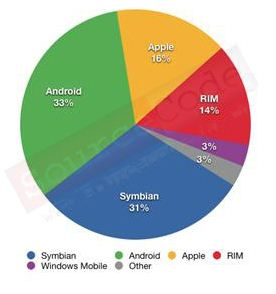
\includegraphics[width=0.5\columnwidth]{Figures/2/maketshare}
%		\caption{ส่วนแบ่งการตลาดระบบปฏิบัติการบนสมาร์ทโฟน}{ที่มา :  https://beerkung.wordpress.com/ระบบปฏิบัติการรุ่นล่าส/ระบบปฏิบัติการ-android.html}
%		\label{Fig:maketshare}
%	\end{figure}
\newpage
	\subsection{ประวัติความเป็นมาของระบบปฏิบัติการแอนดรอยด์}
ถูกพัฒนามาจากบริษัท แอนดรอยด์ (Android Inc.) เมื่อปี พ.ศ 2546 โดยมีนาย แอนดี้ รูบิน (Andy Rubin) ผู้ให้กำเนิดระบบปฏิบัติการนี้ และถูกบริษัท กูเกิ้ล ซื้อกิจการเมื่อ เดือนสิงหาคม ปี พ.ศ 2548 โดยบริษัทแอนดรอยด์ ได้กลายเป็นมาบริษัทลูก ของบริษัทกูเกิ้ล และยังมีนาย แอนดี้ รูบิน ดำเนินงานอยู่ในทีมพัฒนาระบบปฏิบัติการต่อไป
ระบบปฏิบัติการแอนดรอยด์ เป็นระบบปฏิบัติการที่พัฒนามาจากการนำเอา แกนกลางของระบบปฏิบัติการลินุกซ์ (Linux Kernel) ซึ่งเป็นระบบปฏิบัติการที่ออกแบบมาเพื่อทำงานเป็นเครื่องให้บริการ (Server) มาพัฒนาต่อ เพื่อให้กลายเป็นระบบปฏิบัติการบนอุปกรณ์พกพา (Mobile Operating System)
ต่อมาเมื่อเดือน พฤศจิกายน ปี พ.ศ 2550 บริษัทกูเกิ้ล ได้ทำการก่อตั้งสมาคม OHA (Open Handset Alliance) เพื่อเป็นหน่วยงานกลางในการกำหนดมาตรฐานกลาง ของอุปกรณ์พกพาและระบบปฏิบัติการแอนดรอยด์ โดยมีสมาชิกในช่วงก่อนตั้งจำนวน 34 รายเข้าร่วม ซึ่งประกอบไปด้วยบริษัทชั้นนำที่ดำเนินธุรกิจด้าการสื่อสาร เช่น โรงงานผลิตอุปกรณ์พกพา, บริษัทพัฒนาโปรแกรม, ผู้ให้บริการสื่อสาร และผู้ผลิตอะไหล่อุปกรณ์ด้านสื่อสาร \cite{bib2}
% 	\subsection{โครงสร้างของระบบปฏิบัติการแอนดรอยด์}
% 	การทำความเข้าใจโครงสร้างของระบบปฏิบัติการแอนดรอยด์ \cite{androidbook1} ถือว่าเป็นสิ่งสำคัญเพราะถ้านักพัฒนาโปรแกรม สามารถมองภาพโดยรวมของระบบได้ทั้งหมด จะสามารถเข้าใจถึงกระบวนการทำงานได้ดียิ่งขึ้น และสามารถนำไปช่วยในการออกแบบโปรแกรมที่ต้องการพัฒนาเพื่อให้เกิดประสิทธิภาพในการทำงาน
	
% 	\begin{figure}[H]
% 		\centering
% 		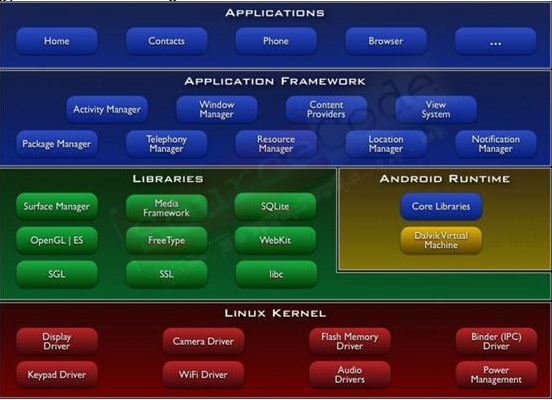
\includegraphics[width=0.8\columnwidth]{Figures/2/androidarchitecture}
% 		\caption{โครงสร้างของระบบปฏิบัติการแอนดรอยด์}{ที่มา : https://www.theandroid-mania.com/android-architecture/}
% 		\label{Fig:androidarchitecture}
% 	\end{figure}
% 	จากโครงสร้างของระบบปฏิบัติการแอนดรอยด์ในรูปที่ \ref{Fig:androidarchitecture} จะสังเกตได้ว่า มีการแบ่งออกเป็นส่วน ๆ ที่มีความเกี่ยวเนื่องกัน โดยส่วนบนสุดเป็นส่วนที่ผู้ใช้งานทำการติดต่อโดยตรงซึ่งคือส่วนของ Applications ลำดับถัดมาเป็นองค์ประกอบอื่น ๆ ตามลำดับ และสุดท้ายเป็นส่วนที่ติดต่อกับอุปกรณ์โดยผ่านทาง Linux Kernel โครงสร้างของแอนดรอยด์สามารถอธิบายได้ดังนี้

% 	\begin{enumerate}
% 		\item Applications ส่วนแอปพลิเคชันหรือส่วนของโปรแกรมที่มากับระบบปฏิบัติการ หรือเป็นกลุ่มของโปรแกรมที่ผู้ใช้งานได้ทำการติดตั้งไว้ โดยผู้ใช้งานสามารถเรียกใช้โปรแกรมต่าง ๆ ได้โดยตรงซึ่งการทำงานของแต่ละโปรแกรมจะเป็นไปตามที่ผู้พัฒนาโปรแกรมได้ออกแบบและเขียนโค้ด (Code) โปรแกรมเอาไว้
% 		\item Application Framework  เป็นส่วนที่มีการพัฒนาขึ้นเพื่อให้นักพัฒนาสามารถพัฒนาโปรแกรมได้สะดวก และมีประสิทธิภาพมากยิ่งขึ้น โดยนักพัฒนาไม่จำเป็นต้องพัฒนาในส่วนที่มีความยุ่งยากมากๆ เพียงแค่ทำการศึกษาถึงวิธีการเรียกใช้งาน Application Framework ในส่วนที่ต้องการใช้งานแล้วนำมาใช้งาน ซึ่งมีหลายกลุ่มด้วยกัน ตัวอย่างเช่น
% 			\begin{itemize}
% 				\item Activities Manager เป็นกลุ่มของชุดคำสั่งที่จัดการเกี่ยวกับวงจรการทำงานของหน้าต่างโปรแกรม (Activity)
% 				\item Content Providers เป็นกลุ่มของชุดคำสั่ง ที่ใช้ในการเข้าถึงข้อมูลของโปรแกรมอื่น และสามารถแบ่งปันข้อมูลให้โปรแกรมอื่นเข้าถึงได้
% 				\item View System เป็นกลุ่มของชุดคำสั่งที่เกี่ยวกับการจัดการโครงสร้างของหน้าจอที่แสดงผลในส่วนที่ติดต่อกับผู้ใช้งาน (User Interface)
% 				\item Telephony Manager เป็นกลุ่มของชุดคำสั่งที่ใช้ในการเข้าถึงข้อมูลด้านโทรศัพท์ เช่น หมายเลขโทรศัพท์ เป็นต้น
% 				\item Resource Manager เป็นกลุ่มของชุดคำสั่งในการเข้าถึงข้อมูลที่เป็นข้อความและรูปภาพ
% 				\item Location Manager เป็นกลุ่มของชุดคำสั่งที่เกี่ยวกับตำแหน่งทางภูมิศาสตร์ที่ระบบปฏิบัติการได้รับค่าจากอุปกรณ์
% 				\item Notification Manager เป็นกลุ่มของชุดคำสั่งที่จะถูกเรียกใช้เมื่อโปรแกรมต้องการแสดงผลให้กับผู้ใช้งาน ผ่านทางแถบสถานะ (Status Bar) ของหน้าจอ
% 			\end{itemize}
% 		\item Libraries เป็นส่วนของชุดคำสั่งที่พัฒนาด้วย C/C++ โดยแบ่งชุดคำสั่งออกเป็นกลุ่มตามวัตถุประสงค์ของการใช้งาน เช่น Surface Manage จัดการเกี่ยวกับการแสดงผล Media Framework จัดการเกี่ยวกับการการแสดงภาพและเสียง Open GL|ES และ SGL จัดการเกี่ยวกับภาพ 3 มิติ และ 2 มิติ SQLlite จัดการเกี่ยวกับระบบฐานข้อมูล เป็นต้น
% 		\item Android Runtime จะมี Darvik Virtual Machine ที่ถูกออกแบบมาเพื่อให้ทำงานบนอุปกรณ์ที่มีหน่วยความจำ (Memmory) หน่วยประมวลผลกลาง (CPU) และพลังงาน (Battery) ที่จำกัดซึ่งการทำงานของ Darvik Virtual Machine จะทำการแปลงไฟล์ที่ต้องการทำงานไปเป็นไฟล์ .DEX ก่อนการทำงานเหตุผลเพื่อให้มีประสิทธิภาพเพิ่มขึ้นเมื่อใช้งานกับหน่วยประมวลผลกลางที่มีความเร็วไม่มากส่วนต่อมาคือ Core Libraries ที่เป็นส่วนรวบรวมคำสั่งและชุดคำสั่งสำคัญโดยถูกเขียนด้วยภาษาจาวา (Java Language)
% 		\item Linux Kernel เป็นส่วนที่ทำหน้าที่หัวใจสำคัญในจัดการกับบริการหลักของระบบปฏิบัติการ เช่น เรื่องหน่วยความจำ พลังงาน ติดต่อกับอุปกรณ์ต่างๆ ความปลอดภัย เครือข่าย โดยแอนดรอยด์ได้นำเอาส่วนนี้มาจากระบบปฏิบัติการลินุกซ์ รุ่น 2.6 (Linux 26. Kernel) ซึ่งได้มีการออกแบบมาเป็นอย่างดี
% 	\end{enumerate}
% %	\subsection{ข้อเด่นของระบบปฏิบัติการแอนดรอยด์}
% %	เนื่องจากระบบปฏิบัติการแอนดรอยด์มีการเจริญเติบโตอย่างรวดเร็วและมีส่วนแบ่งตลาดของอุปกรณ์ด้านนี้ขึ้นทุกขณะ ทำให้กลุ่มผู้ใช้งานและกลุ่มนักพัฒนาโปรแกรมให้ความสำคัญกับระบบปฏิบัติการแอนดรอยด์เพิ่มมากขึ้น
% %	
% %	เมื่อมองในด้านของกลุ่มผลิตภัณฑ์บริษัทที่มีการพัฒนาผลิตภัณฑ์รุ่นใหม่ ได้มีการนำเอาระบบปฏิบัติการแอนดรอยด์ไปใช้ในสินค้าของตนเองพร้อมทั้งยังมีการปรับแต่งให้ระบบปฏิบัติการมีความสามารถ การจัดวาง โปรแกรมและลูกเล่นใหม่ ๆ ที่แตกต่างจากคู่แข่งในท้องตลาดโดยเฉพาะอย่างยิ่งกลุ่มสินค้าที่เป็นมือถือรุ่นใหม่(SmartPhone)และอุปกรณ์จอสัมผัส(Touch Screen)โดยมีลักษณะแตกต่างกันไป เช่น ขนาดหน้าจอ ระบบโทรศัพท์ ความเร็วของหน่วยประมวลผล ปริมาณหน่วยความจำ แม้กระทั่งอุปกรณ์ตรวจจับ(Sensor)ต่าง ๆ 
% %	
% %	หากมองในด้านของการพัฒนาโปรแกรม ทางบริษัท Google ได้มีการพัฒนา Application Framework ไว้สำหรับนักพัฒนาใช้งานได้อย่างสะดวกและไม่เกิดปัญหาเมื่อนำชุดโปรแกรมที่พัฒนาขึ้นมา ไปใช้กับอุปกรณ์ที่มีลักษณะต่างกัน เช่น ขนาดจออุปกรณ์ไม่เท่ากัน ก็ยังสามารถใช้งานโปรแกรมได้เหมือนกัน เป็นต้น
	
% 	\subsection{การจัดการเกี่ยวกับวัฏจักรแอคทิวิตี้ของแอปพลิเคชัน}
	
% 	ขณะที่ผู้ใช้เปิดใช้งานแอปพลิเคชัน -> ออกจากแอปพลิเคชัน -> แล้วก็กลับเข้ามาในแอปพลิเคชันอีกครั้งแอคทิวิตี้จะมีการย้าย Method ต่างๆ เกิดขึ้นในวัฏจักรแอคทิวิตี้ ยกตัวอย่างเช่น 
% 	เมื่อแอคทิวิตี้เริ่มทำงานครั้งแรกจะแสดงขึ้นมาอยู่ด้านบนสุดของระบบ (Foreground) และรอรับการทำงานจากผู้ใช้ในระหว่างกระบวนการนี้ระบบจะมีการเรียกใช้งาน Callback Method หรือ Method ที่ถูกเรียกใช้งานอัตโนมัติในแอคทิวิตี้ที่ได้กำหนดการทำงานให้กับ UI และสวนติดต่ออื่น ๆ ไว้ ถ้าผู้ใช้มีการใช้งานใด ๆ ที่เป็นการเรียกแอคทิวิตี้อื่นขึ้นมาหรือสลับไปใช้งานแอปพลิเคชันอื่นระบบจะเรียก Callback Method อีกอันขึ้นมา เช่น ซ่อนแอปพลิเคชันไว้ด้านหลัง Background (ไม่แสดงแอคทิวิตี้แต่ Instance และ Method นั้นยังทำงานอยู่)
	
% 	ภายใน Callback Method สามารถกำหนดการทำงานในแอคทิวิตี้เมื่อผู้ใช้ออกจากแอปพลิเคชันและกลับเข้ามาใช้งานแอปพลิเคชันใหม่อีกครั้งได้ ตัวอย่าง ถ้าแอปพลิเคชันเป็นแอปพลิเคชัน Streaming Video
% 	อาจจะสั่งให้ทำการหยุด Video ชั่วคราว และปิดการเชื่อมต่อ Network ไว้ก่อนเมื่อผู้ใช้สลับไปใช้แอปพลิเคชันอื่น
% 	และทันทีที่ผู้ใช้กลับมาใช้งานแอปพลิเคชันต่อ ก็ให้ทำการเชื่อมต่อกับ Network และก็อนุญาตให้ผู้ใช้กลับไปเล่น Video
% 	ในตำแหน่งที่ค้างต่อไปทันทีได้โดยที่ไม่ต้องเริ่มต้นแอปพลิเคชันใหม่ เป็นต้น
	
% 	\subsection{กระบวนการเริ่มทำงานของแอคทิวิตี้ (Activity)}
% 	ในระบบแอนดรอย์การกำหนดโค้ดเริ่มต้นไว้ในแอคทิวิตี้โดยสัมพันธ์กับ Method ที่ถูกเรียกใช้งานอัตโนมัติ (Callback Method) อย่างเป็นลำดับ ตั้งแต่เริ่มต้นแอคทิวิตี้ไปจนถึงสิ้นสุดและปิดการทำงานของ Activity ลง
	
% 	\subsection{ทำความรู้จักกับ Lifecycle Callback}
% 	ในขณะที่แอคทิวิตี้ \cite{ActivityLifeCycle} ทำงานระบบจะเรียกใช้ Callback Method ตามลำดับในลักษณะที่คล้ายกับการก่อพีระมิด นั่นคือ แต่ละขั้นตอนวัฏจักรของแอคทิวิตี้คือส่วนแยกย่อยแต่ละขั้นของพีระมิด
% 	เช่น เมื่อระบบสร้าง Instance ของแอคทิวิตี้ขึ้นมาใหม่ Method ที่เรียกใช้งานอัตโนมัติ (Callback Method) จะขยับ Activity Method ขึ้นมาด้านบนโดยด้านบนของพีระมิดคือจุดที่แอคทิวิตี้กำลังทำงานแสดงอยู่ด้านหน้า (Foreground Activity) สุดและผู้ใช้กำลังใช้งานอยู่และเมื่อผู้ใช้กำลังจะออกจากแอคทิวิตี้ระบบจะเรียกใช้ Method อื่นซึ่งทำให้ Activity Method
% 	ถอยกลับไปอยู่ด้านล่างของพีระมิดตามลำดับเพื่อหยุดการทำงานและลบแอคทิวิตี้ออกไป ในบางกรณีแอคทิวิตี้จะย้ายลงมาอยู่บางจุดและรอจังหวะที่จะถูกเรียกกลับขึ้นมาด้านบนอีก เช่น ในกรณีเมื่อผู้ใช้สลับไปใช้งานแอปพลิเคชันอื่นแล้วกลับมาใช้งานอีกครั้ง
% 	\begin{figure}[H]
% 		\centering
% 		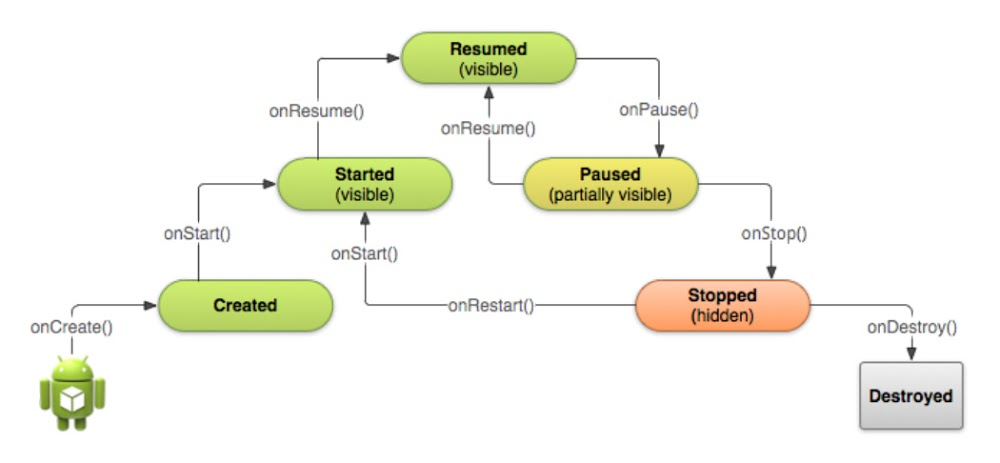
\includegraphics[width=0.8\columnwidth]{Figures/2/lifecycle}
% 		\caption{วัฏจักรของแอคทิวิตี้บนระบบปฏิบัติการแอนดรอยด์}{ที่มา : https://www.dev2qa.com/android-activity-lifecycle-example/}
% 		\label{Fig:lifecycle}
% 	\end{figure}
% 	จากรูปที่ \ref{Fig:lifecycle} แสดงวัฏจักรของแอคทิวิตี้ในรูปแบบโครงสร้างพีระมิดโดยแสดงให้เห็นว่า Method ที่เรียกใช้
% 	งานอัตโมัติ (Callback Method) ได้แก่ onCreate(), onStart(), onResume() และ onRestart() จะขยับแอคทิวิตี้ขึ้นไปด้านบนสุดที่ Resumed Method
% 	และมี Method ได้แก่ onPause(), onStop() และ onDestroy() ที่จะขยับแอคทิวิตี้ลงมาด้านล่าง แอคทิวิตี้ยังสามารถกลับไปทำงานที่ตำแหน่ง Resumed Method จากตำแหน่ง Paused และ Stopped ได้อีกด้วย
	
% 	ในบางครั้งไม่จำเป็นต้องเรียกใช้งาน Callback Method ทั้งหมดเสมอไปขึ้นกับความซับซ้อนของแอคทิวิตี้ อย่างไรก็ตามเป็นสิ่งสำคัญที่นักพัฒนาควรทำความเข้าใจแต่ละ Method เพื่อให้มั่นใจได้ว่าแอปพลิเคชันของที่ได้พัฒนาตอบสนองเป็นไปตามที่ผู้ใช้คาดหวัง ดังนั้น ในการใช้งาน Callback Method
% 	ที่ถูกวิธีก็จะช่วยให้แอปพลิเคชันทำงานได้เป็นอย่างดี ดังนี้
% 	\begin{itemize}
% 		\item ไม่หยุดการทำงานหรือค้าง กรณีมีสายโทรเข้าหรือมีการสลับไปใช้งานแอปพลิเคชันอื่น 
% 		\item ไม่ใช้ทรัพยากรที่มีค่าของระบบอย่างสูญเปล่า ถ้าไม่มีการใช้งานแอคทิวิตี้ใดๆ 
% 		\item ไม่กระทบต่อกระบวนการในขั้นตอนการใช้งานของผู้ใช้กรณีออกจากแอปพลิเคชันแล้วกลับเข้ามาใช้งานอีกครั้ง 
% 		\item ไม่หยุดการทำงานหรือระบบค้างที่กระทบการใช้งานของผู้ใช้กรณีมีการหมุนหน้าจอแนวนอนและแนวตั้งสลับกัน
% 	\end{itemize}
	
% 	เหตุการณ์ที่แอคทิวิตี้มีการเปลี่ยน Method ต่าง ๆ ตามแสดงในรูปที่  \ref{Fig:lifecycle}
% 	แต่มีอยู่ 3 Method เท่านั้นที่แอคทิวิตี้จะยังคงอยู่คงที่ในช่วงเวลาระยะเวลาหนึ่งไม่เปลี่ยนไป Method อื่นในทันที ได้แก่
% 		\begin{itemize}
% 		\item Resumed (แสดงอยู่ ทำงานอยู่) ใน Method นี้แอคทิวิตี้จะแสดงอยู่ด้านหน้าสุดและผู้ใช้กำลังใช้งานอยู่ บ่อยครั้งจะเรียกว่า Running Method
% 		\item Paused (แสดงหน้าจอบางส่วน ไม่ถูกบังสนิท) ใน Method นี้แอคทิวิตี้จะถูกบดบังด้วยแอคทิวิตี้อื่น เช่น แอคทิวิตี้อื่นที่อยู่ด้านหน้าสุดที่แสดงในลักษณะกึ่งโปรงใสหรือไม่ได้แสดงแบบเต็มหน้าจอ  แอคทิวิตี้ในสถานะนี้จะไม่สามารถรับค่าจากผู้ใช้และทำงานคำสั่งใด ๆ ได้
% 		\item Stopped (แสดงหน้าจอแบบ Background ผู้ใช้มองไม่เห็น) ใน Method นี้ แอคทิวิตี้จะถูกบดบังอย่างสมบูรณ์และผู้ใช้มองไม่เห็นโดยจะถูกย้ายไปอยู่ด้านหลังในขณะที่อยู่ใน Method นี้
% 		ค่า Activity Instance และตัวแปรทั้งหมดจะยังคงอยู่แต่จะไม่สามารถถูกเรียกมาใช้งานจากโค้ดใด ๆ ได้
% 		\end{itemize}
% 		ในขณะที่ Method อื่น เช่น Created และ Started จะแสดงชั่วคราวแล้วระบบก็จะเปลี่ยนไป Method อื่นในทันทีที่ Method ถูกเรียกใช้งานอัตโนมัติ นั่นคือ หลังจากที่ระบบเรียกใช้งาน onCreate() แล้วก็จะเรียกใช้งาน onStart()
% 		ทันทีและสุดท้ายตามด้วย onResumne()  ซึ่งก็จะเข้าสู่ Resumed Method ทั้งหมดก็คือวัฏจักรแอคทิวิตี้เบื้อต้น
		
% 	\subsection{การกำหนด Launcher Activity ในแอปพลิเคชัน}
% 	เมื่อผู้ใช้กดที่ Icon App จากหน้า Home Screen เพื่อใช้งาน ระบบก็จะเรียก onCreate() Method
% 	ขึ้นมาทำงานอัตโนมัติเพื่อที่จะเปิดใช้งานแอคทิวิตี้ที่ได้กำหนดให้เป็นแอคทิวิตี้หลัก ("launcher" หรือ "main" ) 
% 	ซึ่งก็จะเป็นแอคทิวิตี้ที่เป็นหน้าหลักที่ผู้ใช้จะเห็นเมื่อเข้ามาใช้งานแอปพลิเคชัน สามารถกำหนดได้ว่าแอคทิวิตี้ใดที่จะใช้เป็น Activity หลักโดยกำหนดค่าในไฟล์ AndroidManifest.xml
	
% 	แอคทิวิตี้หลักจะต้องกำหนด ค่าใน manifest ด้วย <intent-filter> 
% 		\begin{figure}[H]
% 			{\setstretch{1.0}\begin{lstlisting}
% <intent-filter>
% <action android:name="android.intent.action.MAIN" />
% <category android:name="android.intent.category.LAUNCHER" />
% </intent-filter>
% 					\end{lstlisting}}
% 					\caption{การกำหนด Launcher Activity ในแอปพลิเคชัน}
% 					\label{Fig:Launcher}
% 		\end{figure}
% โดยประกอบไปด้วย MAIN action และ LAUNCHER category ดังตัวอย่างดังนี้
% 				\begin{figure}[H]
% 					{\setstretch{1.0}\begin{lstlisting}
% <Activity android:name=".MainActivity" android:label="@string/app_name">
% <intent-filter>
% <action android:name="android.intent.action.MAIN" />
% <category android:name="android.intent.category.LAUNCHER" />
% </intent-filter>
% </Activity>
% 						\end{lstlisting}}
% 					\caption{การกำหนด Launcher Activity ในแอปพลิเคชัน}
% 					\label{Fig:category}
% 				\end{figure}
%    ใน Android Studio เมื่อสร้างโปรเจค (Project) ขึ้นมาจะมีการประกาศค่าและกำหนดให้มีการเรียกใช้งาน filter ในไฟล์ AndroidManifest.xml มาให้เรียบร้อยแล้ว ถ้าไม่ได้กำหนด MAIN action และ LAUNCHER category แล้ว App Icon ของจะไม่แสดงในหน้าหลักของลิสรายการแอปพลิเคชันบนหน้าจอสมาร์ทโฟนของผู้ใช้
% 	\subsection{การสร้าง Instance ใหม่}
% 	แอปพลิเคชันส่วนใหญ่จะประกอบไปด้วยแอคทิวิตี้หลายอันทำงานแตกต่างกันไป  ไม่ว่าจะเป็นแอคทิวิตี้หลักที่ถูกสร้างขึ้นเมื่อผู้ใช้คลิกที่ icon app หรือแอคทิวิตี้ต่าง ๆ ที่ถูกเรียกใช้งานโดยผู้ใช้ ทั้งหมดล้วนแล้วเป็นสิ่งที่ระบบสร้าง instance ใหม่ของแอคทิวิตี้โดยการเรียกใช้ผ่าน onCreate() Method ต้องใช้ onCreate() Method ในเหตุผลเพื่อเริ่มต้นแอปพลิเคชันซึ่งควรจะเกิดขึ้นเพียงครั้งเดียวตลอดหนึ่งวัฏจักรของแอคทิวิตี้เช่น ใช้ onCreate() กำหนดหน้าตาของแอปพลิเคชันหรือประกาศตัวแปรที่จะถูกใช้งานในคลาส (Class) เป็นต้น ตัวอย่างการใช้งาน onCreate() Method ตามตัวอย่างรูปที่ \ref{Fig:onCreate} แสดง code เพื่อให้เห็นการตั้งค่าเบื่องต้นเช่น การกำหนด User interface(โดยใช้ XML layout ไฟล์) การประกาศตัวแปรต่าง ๆ การตั้งค่ากำหนดเงื่อนไข UI 
% 					\begin{figure}[H]
% 						{\setstretch{1.0}\begin{lstlisting}
% TextView mTextView; // การประกาศตัวแปรจำหรับ text view ใน layout

% @Override
% public void onCreate(Bundle savedInstanceMethod) {
% 	super.onCreate(savedInstanceMethod);

% // การกำหนด user interface (โดยใช้ XML layout ไฟล์) 
% // ไฟล์ layout ใน project จะอยู่ที่  res/layout/main_Activity.xml 
% 	setContentView(R.layout.main_Activity);

% // กำหนดค่าให้กับ TextView ดังนั้นสามารถเรียกใช้งานผ่านชื่อตัวแปรได้ภายหลัง
% 	mTextView = (TextView) findViewById(R.id.text_message);

% // ตั้งค่าสำหรับกำหนดเงื่อนไข UI 
% // ตรวจสอบเพื่อยืนยันว่ากำลังใช้งานบน android  Honeycomb   
% // หรือสูงกว่า เพื่อเรียกใช้ ActionBar API  
% 	if (Build.VERSION.SDK_INT >= Build.VERSION_CODES.HONEYCOMB) {
% 		// กำหนดให้ icon ใน action bar ไม่ทำงานคล้ายปุ่ม Home  
% 		ActionBar actionBar = getActionBar();
% 		actionBar.setHomeButtonEnabled(false);
% 	}
% }
% 							\end{lstlisting}}
% 						\caption{การใช้งาน onCreate()}
% 						\label{Fig:onCreate}
% 					\end{figure}
% 		เมื่อ onCreate() ทำงานเสร็จระบบจะเรียก onStart() และ onResume() memthod มาทำงานต่อในทันที แอคทิวิตี้จะไม่อยู่ใน Created Method หรือ Started Method ในทางเทคนิคแอคทิวิตี้จะแสดงขึ้นมาทันทีที่ onStart() ถูกเรียกใช้งานแต่ onResume() จะแสดงตามมาติด ๆ ในทันทีและจะอยู่ใน Resumed Method จนกว่าจะมีการเปลี่ยนแปลงบางอย่างเกิดขึ้นเช่น มีสายโทรเข้าหรือผู้ใช้เปิดไปแอคทิวิตี้อื่นหรือปิดหน้าจอลง
		
% 		 โครงสร้างของวัฏจักรแอคทิวิตี้ที่เน้นไปที่ 3 Method หลักที่ระบบเรียกใช้อัตโนมัติตามลำดับ เมื่อมีการสร้าง Instance
% 		 ของแอคทิวิตี้ขึ้นมาใหม่ ได้แก่ onCreate(), onStart() และ onResume() เมื่อลำดับการทำงานเสร็จสิ้นลงแอคทิวิตี้จะ
% 		 มาอยู่ที่ Resumed Method ซึ่งผู้ใช้ใช้งานอยู่จนกว่าจะเปลี่ยนไปเรียกใช้งานแอคทิวิตี้อื่นขึ้นมา
		 
% 	\subsection{การสิ้นสุดการทำงานของแอคทิวิตี้ (Destroy Activity)}
% 	ในขณะที่วัฏจักรของแอคทิวิตี้มี Method แรกคือ onCreate() และ Method สุดท้ายคือ onDestroy()
% 	ระบบจะเรียก Method นี้ในแอคทิวิตี้เป็นสัญญาณว่า Activity instance นี้จะถูกลบบออกอย่างสมบูรณ์จากหน่วยความจำของระบบ (System memory)
	
% 	แอปพลิเคชันส่วนใหญ่ไม่จำเป็นต้องกำหนด Method นี้เพราะ local class ถูกทำลายไปพร้อมกับแอคทิวิตี้และแทบจะถูกลบไปอย่างสมบูร์ในระหว่างเรียกใช้งาน onPause() และ onStop() อย่างไรก็ตามถ้าแอคทิวิตี้ของมีการกำหนดให้มีการทำงานแบบ background (ทำงานอยู่เบื้องหลัง) ในขั้นตอน onCreate() ด้วยแล้วหรือมีการใช้งานทรัพยากรของระบบเป็นระยะเวลานานเป็นเหตุให้ความจำถูกใช้งานจำนวนมาก หากไม่ทำการปิดการใช้งาน จึงควรอย่างยิ่งที่จะเรียกใช้งาน Method onDestroy() เพื่อคืนค่าหน่วยความจำให้ระบบ
% 						\begin{figure}[H]
% 							{\setstretch{1.0}\begin{lstlisting}
% @Override
% public void onDestroy() {
% 	super.onDestroy();  // เรียกใช้งาน superclass ทุกครั้งเสมอ

% // หยุดการติดตามหรือตรวจจับ Method ของ Activity 
% 	android.os.Debug.stopMethodTracing();
% }
% 								\end{lstlisting}}
% 							\caption{การใช้งาน onDestroy()}
% 							\label{Fig:onDestroy}
% 						\end{figure}
% 	ระบบจะเรียกใช้งาน onDestroy() หลังจากเรียกใช้งาน onPause() และ onStop() แล้วในทุกเหตุการณ์ ยกเว้นกรณีมีการกำหนดให้เรียกใช้ finish() ภายใน onCreate() Method ในกรณีเช่น Activity หยุดชั่วคราวเพื่อทำการเรียกใช้งานแอคทิวิตี้อื่นข้ามาแล้วทำการกำหนดให้มีการเรียกใช้งาน finish() ที่กำหนดใน onCreate() Method เพื่อทำลายแอคทิวิตี้ในกรณีนี้ระบบจะทำการเรียก onDestroy() ทันทีโดยไม่ผ่าน Callback Method อื่นเช่น ไม่ผ่าน onPause() หรือ onStop() แบบนี้เป็นต้น
\newpage

\section{ความรู้พื้นฐาน Java}
Java \cite{java} เป็นภาษาเขียนโปรแกรมเพื่อวัตถุประสงค์ทั่วไป โดยสามารถทำงานได้พร้อมกัน เป็นภาษาที่สร้างมาจากคลาส และสนับสนุนการเขียนโปรแกรมแบบออบเจ็คอย่างสมบูรณ์ และถูกออกแบบมาให้พร้อมสำหรับการใช้งานมากที่สุด ซึ่งมีเมธอดและคลาสต่าง ๆ อำนวยความสะดวกให้ใช้มากมาย โดยภาษา Java นั้นมีความตั้งใจว่าจะทำให้นักพัฒนาออกแบบและพัฒนาโปรแกรมน้อยลง นั่นคือการเขียนเพียงครั้งเดียว แต่นำไปใช้งานได้ทุกที่หรือทุกแพลตฟอร์ม

แอปพลิเคชันของภาษา Java นั้นโดยปกติแล้วจะคอมไพล์เป็น bytecode ที่สามารถรันได้ใน Java virtual machine (JVM) ขึ้นกับสถาปัตยกรรมของคอมพิวเตอร์นั้นๆ และใน ปี 2016 ภาษา Java เป็นภาษาที่ได้รับความนิยมและใช้มากที่สุดในโลก โดยเฉพาะการใช้พัฒนาเว็บแอปพลิเคชัน

	\subsection{ประวัติความเป็นมาของภาษา Java}
	James Gosling Mike Sheridan และ Patrick Naughton ได้เริ่มก่อตั้งโปรเจ็คภาษา Java เมื่อปี 1991 โดยในตอนแรกถูกพัฒนาสำหรับทีวีที่สามารถมีปฎิสัมพันธ์ได้ เช่น เล่นเกมในทีวี แต่ประสบปัญหาในการที่จะใช้งานกับสายเคเบิลของทีวีดิจิตอล ในตอนแรกภาษา Java ใช้ชื่อว่า Oak เพราะว่ามีต้นโอ็คยื่นออกไปยังออฟฟิศของ Gosling ต่อมาใช้ชื่อว่า Green และในตอนท้ายใช้ชื่อว่า Java มีที่มาจากกาแฟ Java 
	
	ภาษาได้รับการออกแบบให้มีรูปแบบทางภาษาเหมือนภาษา C และ C++ ซึ่งทำให้โปรแกรมเมอร์ส่วนมากนั้นคุ้นเคยกับมันได้ดีขึ้น และ Sun Microsystems เผยแพร่ Java 1.0 ในปี 1995 โดยมีคำกล่าวว่า "Write Once, Run Anywhere" (WORA)  เขียนเพียงครั้งเดียวและสามารถนำไปใช้งานได้บนทุกแพลตฟอร์ม

	\section{ความรู้พื้นฐาน Python}
	Python \cite{py} เป็นภาษาเขียนโปรแกรมระดับสูงที่ใช้กันอย่างกว้างขวางในการเขียนโปรแกรมสำหรับวัตถุประสงค์ทั่วไป 
	ภาษา Python นั้นสร้างโดย Guido van Rossum และถูกเผยแพร่ครั้งแรกในปี 1991 Python 
	นั้นเป็นภาษาแบบ interprete ที่ถูกออกแบบโดยมีปรัญชาที่จะทำให้โค้ดอ่านได้ง่ายขึ้น
	 และโครงสร้างของภาษานั้นจะทำให้โปรแกรมเมอร์สามารถเข้าใจแนวคิดการเขียนโค้ดโดยใช้บรรทัดที่น้อยลงกว่าภาษาอย่าง 
	 C++ และ Java ซึ่งภาษานั้นถูกกำหนดให้มีโครงสร้างที่ตั้งใจให้การเขียนโค้ดเข้าใจง่ายทั้งในโปรแกรมเล็กไปจนถึงโปรแกรมขนาดใหญ่
	 
	\subsection{ประวัติความเป็นมาของภาษา Python}
	Python กำเนิดขึ้นตั้งแต่ 1980 
	และเริ่มต้นใช้งานกันช่วงธันวาคม 1989 โดยนาย
	Gudio Van Rossum
	 ภายใต้ Centrum Wiskunde and Informatica (CWI) ที่ Netherlands\cite{bpy}	
% 	\subsection{Java Compiler}
% 	ในการเขียนโปรแกรมในภาษา Java ต้องการ Java Compiler เพื่อทำการแปลงโค้ดของโปรแกรมที่เขียนเป็น bytecode เพื่อนนำไปรันในแต่ละแพลตฟอร์มต่อไป โดยเรียกว่า Java Platform (JDK) ซึ่งประกอบไปด้วยคอมไพล์เลอร์ ในการแปลงโค้ดภาษา Java ให้เป็น Bytecode และ Java virtual machine (JVM) สำหรับรันโปรแกรมของภาษา Java ในแต่ละแพลตฟอร์ม สำหรับในบทเรียนนี้จะใช้ IDE ในการพัฒนาเพื่อความสะดวกและรวดเร็ว
	
% 	\subsection{โครงสร้างของภาษา Java}

%   \begin{figure}[H]
%     \begin{minted}[frame=lines,framesep=2mm,baselinestretch=1.15,fontsize=\footnotesize,linenos]{java}
%     public class ClassName {
%       public static void main(String[] args) {
%         System.out.println("Hello สวัสดี");
%       }
%     }
%     \end{minted}
%     \caption{ตัวอย่างโปรแกรมภาษา Java ด้วย minted}
%     \label{Fig:JavaClassMinted}
%   \end{figure}
  
%   รูปที่ \ref{Fig:JavaClassMinted} แสดงให้เห็นผลลัพธ์ของการใช้ minted เพื่อแสดงคำสั่งในเอกสาร Latex

% 	\begin{itemize}
% 		\item Package เป็นกลุ่มของคลาสหรือไลบรารี่มาตรฐานของภาษา Java ที่มีฟังก์ชันต่าง ๆ ให้ใช้มากมาย
% 		\item Class ในส่วนของการประกาศคลาส จะต้องประกาศคลาสให้ชื่อตรงกับไฟล์เสมอ นอกจาก Inner คลาสที่อยู่ในคลาสเดียวกัน โดยชื่อคลาสนั้นควรจะขึ้นต้นด้วยตัวใหญ่และถ้ามีหลายคำให้ใช้ตัวพิมพ์ใหญ่แบ่ง ดังตัวอย่างในรูปที่ \ref{Fig:ClassName}
% 				\begin{figure}[H]
% 					{\setstretch{1.0}\begin{lstlisting}
% public class ClassName {
% ...
% }
% 						\end{lstlisting}}
% 					\caption{การงประกาศคลาสในภาษา Java}
% 					\label{Fig:ClassName}
% 				\end{figure}
% 			\item Method หลังจากคลาสสร้างแล้ว จะเป็นประกาศเมธอดภายในคลาส โดยในการที่จะรันโปรแกรมได้จะต้องมีเมธอดที่ชื่อว่า Main ดังตัวอย่างในโปรแกรมด้านบน มันเป็นที่แรกที่โปรแกรมจะเริ่มทำงาน \ref{Fig:ClassName}
% 			\begin{figure}[H]
% 				{\setstretch{1.0}\begin{lstlisting}
% public static void main (String[] args) {
% ...
% }
% 					\end{lstlisting}}
% 				\caption{การงประกาศเมธอด main ในภาษา Java}
% 				\label{Fig:main}
% 			\end{figure}
% 			\item Methodments เป็นคำสั่งของโปรแกรมเพื่อให้โปรแกรมทำงานตามต้องการ เช่น System.out.println("Hello World!"); เป็นการแสดงผลข้อความออกทางหน้าจอ โดยปกติโปรแกรมมักจะมีหลายคำสั่ง
% 			\item Semicolon ทุกคำสั่งการทำงานของโปรแกรมในภาษา Java จะจบด้วยเครื่องหมาย Semicolon (;) นั่นหมายความว่าสามารถเขียนโปรแกรมแบบไหนก็ได้ โดยคอมไพเลอร์จะทราบอัตโนมัติว่าสิ้นสุดคำสั่งที่ไหน
% 			\item ในภาษา Java สามารถใช้ White space ได้อย่างอิสระตามที่ต้องการ โดย White space จะประกอบไปด้วย Space bar Tab และ Enter (return) เพราะว่าคอมไพเลอร์ตรวจการสิ้นสุดของคำสั่งด้วย ; ใช้ while space ทำให้โค้ดอ่านเข้าใจง่าย และเป็นระเบียบ
% 			\item Literals คือค่าของข้อมูลใดๆ ที่กำหนดให้กับตัวแปรได้ เรียกว่า Constant Literals ทุกค่าที่เป็นไปได้ เช่น "MarcusCode" เป็น String Literals 10 เป็น Integer Literals หรือ true เป็น Boolean Literals โดย Literals เป็นได้แค่ Primitive data type เท่านั้น ตัวอย่างการกำหนดค่าหรือ Literals ให้กับตัวแปร
% 			\item Expression เป็นการกระทำระหว่างตัวแปรกับตัวดำเนินการเพื่อให้ได้ผลลัพธ์ใหม่ เช่น 4 + 3 เป็น expression ของการบวกเลขและได้ได้ผลลัพธ์เท่ากับ 7 หรือ 1 == 1 เป็น expression ของการเปรียบเทียบระหว่างค่าสองค่าว่าเท่ากันหรือไม่ และได้ผลลัพธืเป็น true
% 			\item Keyword คือคำที่สงวนไว้ในภาษา Java นั่นหมายความว่าไม่สามารถนำคำเหล่านี้ไปประกาศเป็นชื่อตัวแปร เมธอด หรือว่าคลาสได้ เพราะว่า Keyword ถูกใช้โดยคอมไพเลอร์เพื่อให้มันทำงานได้สมบูรณ์
% 		\end{itemize}
	

	 
	 \section{ความรู้พื้นฐาน Tensorflow Lite}
	 Tensorflow Lite คือ Library ที่ถูก optimize จาก Tensorflow ทำให้มีขนาดเล็กลงทำให้สามารถทำงานบนอุปกรณ์พกพาได้ ใช้สำหรับพัฒนา Machine Learning Deep Learning และ Neural Network ได้รับการพัฒนาโดยบริษัท Google 
	 ได้ทำการเปิดตัวในงาน I/O ปี 2017 รองรับระบบปฏิบัติการ Android และ IOS ลำดับชั้นในการเรียกใช้ TensorFlow Lite แอพจะเรียกใช้งานผ่านเอนจิน TensorFlow Lite ที่ฝังมาในตัวแอปพลิเคชัน จากนั้น TensorFlow Lite จะเรียกใช้ฟีเจอร์ Android Neural Networks (Android NN) ของ ระบบปฏิบัติการ ที่เริ่มมีการใส่เข้ามาใน Android 8.1
	ลำดับสุดท้าย Android Neural Network จะเรียกใช้ตัวเร่งการประมวลผลที่ระดับฮาร์ดแวร์ 
%			\begin{figure}[H]
%				\centering
%				
\includegraphics[width=0.4\columnwidth]{Figures/2/vuelogo}
%				\caption{ตราสัญลักษณ์ของวิวเจเอส}{ที่มา : https://seeklogo.com/vector-logo/274070/vue-js}
%				\label{Fig:oop}
%			\end{figure}
%		\subsection{ภาพรวมของ Vue.js}
		
	
    \section{ความรู้พื้นฐาน Image Processing}
		Image Processing \cite{imgp} หรือ การประมวลผลภาพดิจิทัล เป็นการแปลงข้อมูลรูปที่เป็นสัญญาณแอนะล็อกให้อยู่ในรูปของสัญญาณดิจิทัล เพื่อใช้ในการประมวลผลผ่านทางคอมพิวเตอร์ได้ และ ยังนำมาใช้ในการลดปัญหาของภาพเช่น ลดสัญญาณรบกวนภายในภาพเป็นต้น

		ในการแปลงภาพให้เป็นสัญญาณดิจิทัลนั้น ระบบจะนำรูปที่รับเข้ามาไปคำนวณ โดยกระบวนการSampling และ Quantization และส่งข้อมูลออกมาในรูปแบบดิจิทัล คอมพิวเตอร์จะเก็บข้อมูลภาพลงหน่วยความจำ โดยการจองหน่วยความจำภายในเครื่องในรูปแบบของอาร์เรย์ โดยค่าในแต่ละช่องของ อาร์เรย์แสดงถึงคุณสมบัติต่างๆของรูปที่จุด พิกเซล นั้นๆ และตำแหน่งของช่อง อาร์เรย์ก็เป็นตัวกำหนดตำแหน่งของจุด พิกเซล ภายในภาพด้วย
		
		\begin{figure}[H]
			\centering
			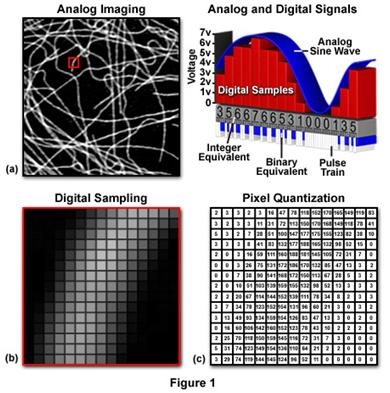
\includegraphics[width=0.8\textwidth]{Figures/2/1.jpg}
			\caption{การแปลงภาพแอนะล็อกให้เป็นภาพดิจิทัล}{ที่มา : https://nextsoftwares.wordpress.com/2014/05/22/}
			\label{Fig:Studentloan1}
		\end{figure}
		ภาพดิจิทัลที่ได้จะมีรูปแบบการเก็บเป็นเมทริกซ์ ซึ่งจะมีการจัดเก็บภาพแต่ละชนิดต่างกัน ขึ้นอยู่กับระบบสีของภาพดังกล่าว โดยแบ่งชนิดของภาพได้ดังนี้
		   \begin{itemize}
			   	\item   Binary imageหรือ ภาพขาว-ดำ เป็นรูปที่ใช้เนื้อที่เพียง 1 บิต ต่อ พิกเซล โดยค่าสีจะมีแค่สองค่าคือ 0 หรือสีดำ และ 1 หรือสีขาว
				 
					 \begin{figure}[H]
						\centering
						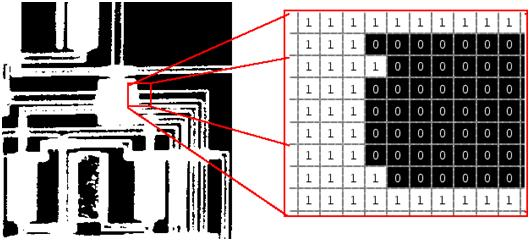
\includegraphics[width=0.8\textwidth]{Figures/2/2.jpg}
						\caption{ภาพแบบ Binary หรือ ภาพขาว-ดำ}{ที่มา : https://nextsoftwares.wordpress.com/2014/05/22/}
						\label{Fig:Studentloan1}
					\end{figure}

						\item  Grayscale Image เป็นรูปที่เก็บโดยใช้รูปแบบของอาร์เรย์ 2 มิติ โดยค่าที่เก็บจะมีค่าอยู่ในช่วงๆหนึ่ง ซึ่งระดับของสีขึ้นอยู่กับขนาดของบิตที่ใช้เก็บค่าสี

						\begin{figure}[H]
							\centering
							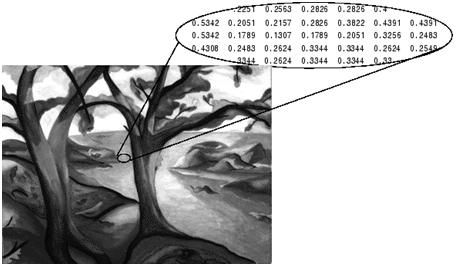
\includegraphics[width=0.8\textwidth]{Figures/2/3.jpg}
							\caption{ภาพแบบ Grayscale}{ที่มา : https://nextsoftwares.wordpress.com/2014/05/22/}
							\label{Fig:Studentloan1}
						\end{figure}
								\item RGB Image หรือ Truecolor Image เป็นรูปที่เก็บโดยใช้อาร์เรย์ 3 มิติ ขนาด m x n x 3 โดยที่ m คือความยาว และ n คือความกว้างของภาพในหน่วยพิกเซล ส่วนมิติสุดท้ายนั้น ในแต่ละมิติจะเก็บค่าสีแยกกัน คือสีแดง(Red) สีเขียว(Green) และสีน้ำเงิน(Blue)
							\begin{figure}[H]
									\centering
									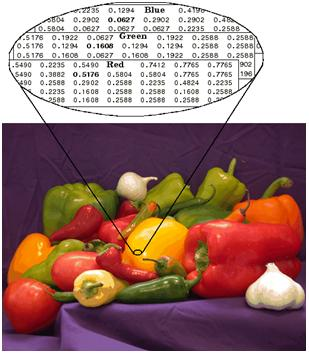
\includegraphics[width=0.4\textwidth]{Figures/2/4.jpg}
									\caption{ภาพแบบ RGB}{ที่มา : https://nextsoftwares.wordpress.com/2014/05/22/}
									\label{Fig:Studentloan1}
								\end{figure}
					
									\item  Indexed Image เป็นรูปที่มีรูปแบบการเก็บแบบ indexed คือ ภาพประเภทนี้จะเก็บค่าสีเป็น indexed และในแต่ละช่องอาร์เรย์ จะเก็บตำแหน่งของสีใน indexed นั้นๆไว้

									\begin{figure}[H]
										\centering
										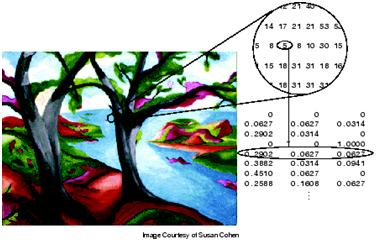
\includegraphics[width=0.8\textwidth]{Figures/2/6.jpg}
										\caption{ภาพNeural Network โครงข่ายประสาทเทียม}{ที่มา : https://nextsoftwares.wordpress.com/2014/05/22/}
										\label{Fig:Studentloan1}
									\end{figure}

								\end{itemize}

								\section{ความรู้พื้นฐาน ปัญญาประดิษฐ์}
								ปัญญาประดิษฐ์ \cite{AI} หรือ Artificial Intelligence  เป็นศาสตร์แขนงหนึ่งของวิทยาศาสตร์คอมพิวเตอร์ ที่เกี่ยวข้องกับวิธีการทำให้คอมพิวเตอร์มีความสามารถคล้ายมนุษย์หรือเลียนแบบพฤติกรรมมนุษย์ คือโปรแกรม Software (ซอฟแวร์) ต่าง ๆ ที่ใช้กับคอมพิวเตอร์ โดยเฉพาะความสามารถในการคิดเองได้ หรือมีปัญญานั่นเอง ปัญญานี้มนุษย์เป็นผู้สร้างให้คอมพิวเตอร์ จึงเรียกว่า ปัญญาประดิษฐ์ 
	 คำนิยาม AI ตามความสามารถที่มนุษย์ต้องการแบ่งได้ 4 กลุ่ม ดังนี้
	 \begin{itemize}
		\item  การกระทำคล้ายมนุษย์ Acting Humanly การสร้างเครื่องจักรที่ทำงาน, สามารสื่อสารได้ด้วยภาษาที่มนุษย์ใช้ เช่น ภาษาไทย ภาษาอังกฤษ เช่น การแปลงข้อความเป็นคำพูด และ การแปลงคำพูดเป็นข้อความ, 
		มีประสาทรับสัมผัสคล้ายมนุษย์ เช่น คอมพิวเตอร์รับภาพได้โดยอุปกรณ์รับสัมผัส แล้วนำภาพไปประมวลผล,เคลื่อนไหวได้คล้ายมนุษย์ เช่น หุ่นยนต์ช่วยงานต่าง ๆ อย่างการ ดูดฝุ่น เคลื่อนย้ายสิ่งของ และเรียนรู้ได้ โดยสามารถตรวจจับรูปแบบการเกิดของเหตุการณ์ใด ๆ แล้วปรับตัวสู่สิ่งแวดล้อมที่เปลี่ยนไปได้
		\item  การคิดคล้ายมนุษย์ Thinking Humanly  กลไกของกิจกรรมที่เกี่ยวข้องกับความคิดมนุษย์ เช่น การตัดสินใจ การแก้ปัญหา การเรียนรู้
		\item  คิดอย่างมีเหตุผล Thinking rationally การศึกษาความสามารถในด้านสติปัญญาโดยการใช้โมเดลการคำนวณ, การศึกษาวิธีการคำนวณที่สามารถรับรู้ ใช้เหตุผล และกระทำ และใช้หลักตรรกศาสตร์ในการคิดหาคำตอบอย่างมีเหตุผล เช่น ระบบผู้เชี่ยวชาญ
		\item กระทำอย่างมีเหตุผล Acting rationally การศึกษาเพื่อออกแบบโปรแกรมที่มีความสามารถในการกระทำ หรือเป็นตัวแทนในระบบอัตโนมัติต่าง ๆ ที่มีปัญญา, พฤติกรรมที่แสดงปัญญาในสิ่งที่มนุษย์สร้างขึ้น และการเพื่อบรรลุเป้าหมายที่ได้ตั้งไว้ เช่น โปรแกรมเล่นเกมหมากรุก ที่จะทำให้คู่ต่อสู้แพ้ให้ได้
		
	\end{itemize}
	% \section{ความรู้พื้นฐาน โครงข่ายประสาทเทียม }
	% โครงข่ายประสาทเทียม  \cite{vuejs} หรือ Artificial Neural Networks คือโมเดลทางคณิตศาสตร์ สำหรับประมวลผลสารสนเทศด้วยการคำนวณแบบคอนเนคชันนิสต์ (Connectionist) เพื่อจำลองการทำงานของเครือข่ายประสาทในสมองมนุษย์ ด้วยวัตถุประสงค์ที่จะสร้างเครื่องมือซึ่งมีความสามารถในการเรียนรู้การจดจำรูปแบบ(Pattern Recognition) และการสร้างความรู้ใหม่ (Knowledge Extraction)
	% เช่นเดียวกับความสามารถที่มีในสมองมนุษย์ สำหรับในคอมพิวเตอร์ Neurons ประกอบด้วย input และ output เหมือนกัน โดยจำลองให้ input แต่ละอันมี weight เป็นตัวกำหนดน้ำหนักของ input โดย neuron แต่ละหน่วยจะมีค่า threshold เป็นตัวกำหนดว่าน้ำหนักรวมของ input ต้องมากขนาดไหนจึงจะสามารถส่ง output ไปยัง neurons ตัวอื่นได้ เมื่อนำ neuron แต่ละหน่วยมาต่อกันให้ทำงานร่วมกันการทำงานนี้ในทางตรรกแล้วก็จะเหมือนกับปฏิกิริยาเคมีที่เกิดในสมอง		

	% \begin{figure}[H]
	% 	\centering
	% 	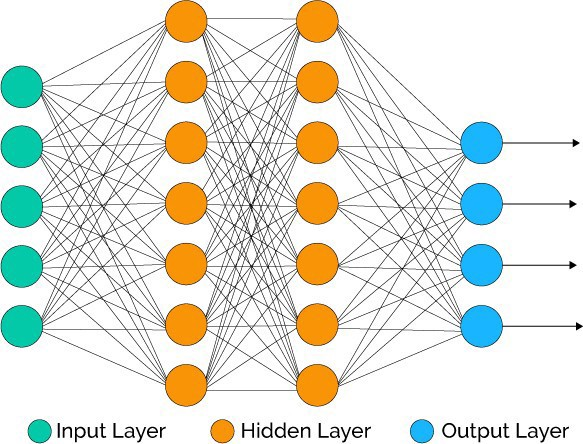
\includegraphics[width=0.4\textwidth]{Figures/2/9.jpeg}
	% 	\caption{Neural Network โครงข่ายประสาทเทียม}{ที่มา :  https://towardsdatascience.com/machine-learning-fundamentals-ii-neural-networks-f1e7b2cb3eef}
	% 	\label{Fig:Studentloan1}
	% \end{figure}
	% \subsection{การเรียนรู้ของ โครงข่ายประสาทเทียม}
	% 		การเรียนรู้ของโครงข่ายประสาทเทียมแบ่งได้ 2 ประเภทดังนี้
	% 		\begin{itemize}
	% 			\item Supervised Learning การเรียนแบบมีการสอน
	% 			เป็นการเรียนแบบที่มีการตรวจคำตอบเพื่อให้โครงข่ายประสาทเทียมปรับตัว ชุดข้อมูลที่ใช้สอนโครงข่ายประสาทเทียมจะมีคำตอบไว้คอยตรวจดูว่าโครงข่ายประสาทเทียมให้คำตอบที่ถูกหรือไม่ ถ้าตอบไม่ถูก โครงข่ายประสาทเทียมก็จะปรับตัวเองเพื่อให้ได้คำตอบที่ดีขึ้น 
				
	% 			\begin{figure}[H]
	% 				\centering
	% 				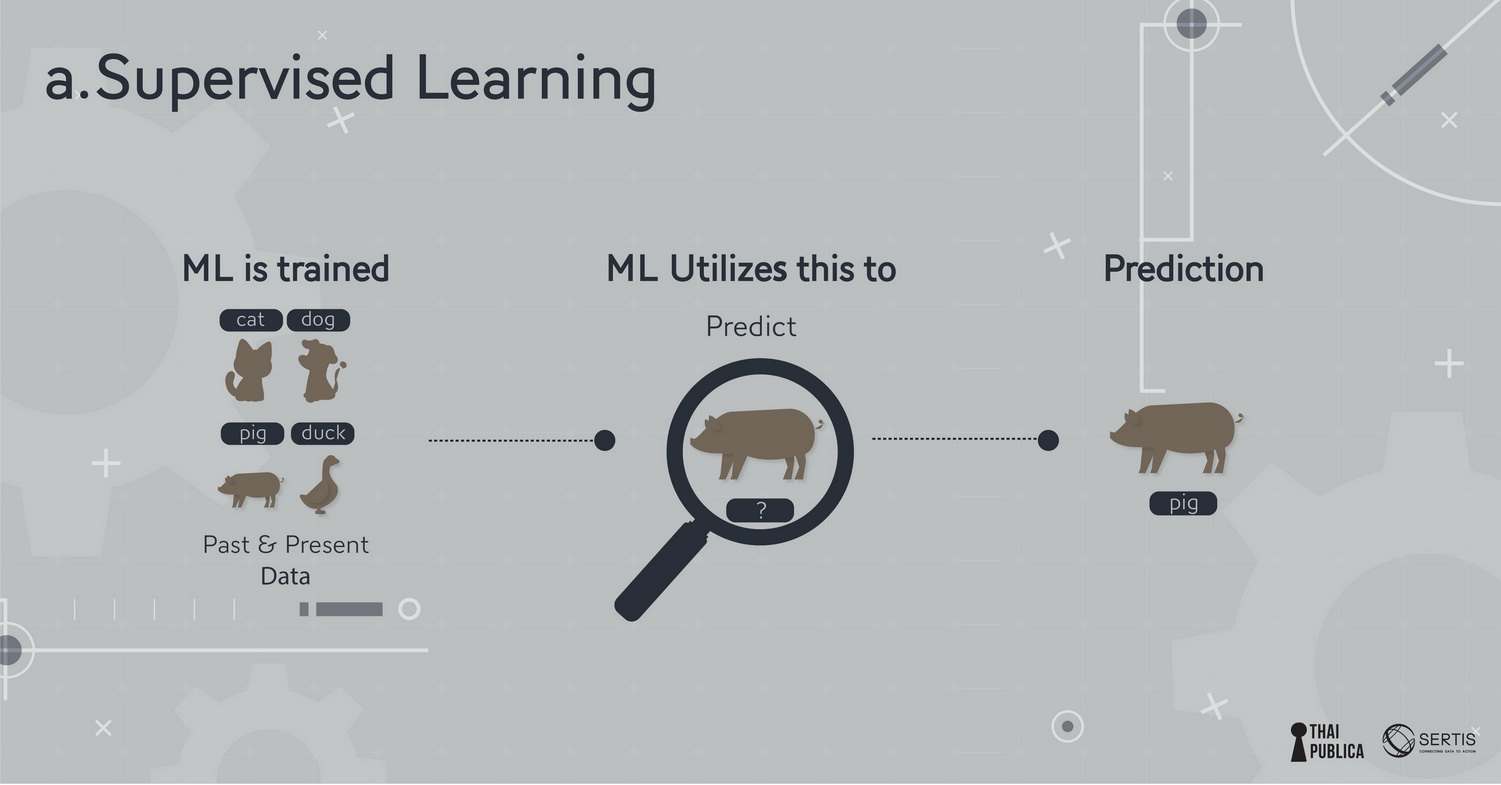
\includegraphics[width=0.8\textwidth]{Figures/2/7.jpg}
	% 				\caption{โมเดลที่ถูกสอนแบบ supervised learning}{ที่มา : https://thaipublica.org/2017/07/data-driven-society12/}
	% 				\label{Fig:Studentloan1}
	% 			\end{figure}
				
	% 			\item  Unsupervised Learning การเรียนแบบไม่มีการสอน
	% 			เป็นการเรียนแบบไม่มีผู้แนะนำ ไม่มีการตรวจคำตอบว่าถูกหรือผิด โครงข่ายประสาทเทียมจะจัดเรียงโครงสร้างด้วยตัวเองตามลักษณะของข้อมูล ผลลัพธ์ที่ได้ โครงข่ายประสาทเทียมจะสามารถจัดหมวดหมู่ของข้อมูลได้ 
	% 			\begin{figure}[H]
	% 				\centering
	% 				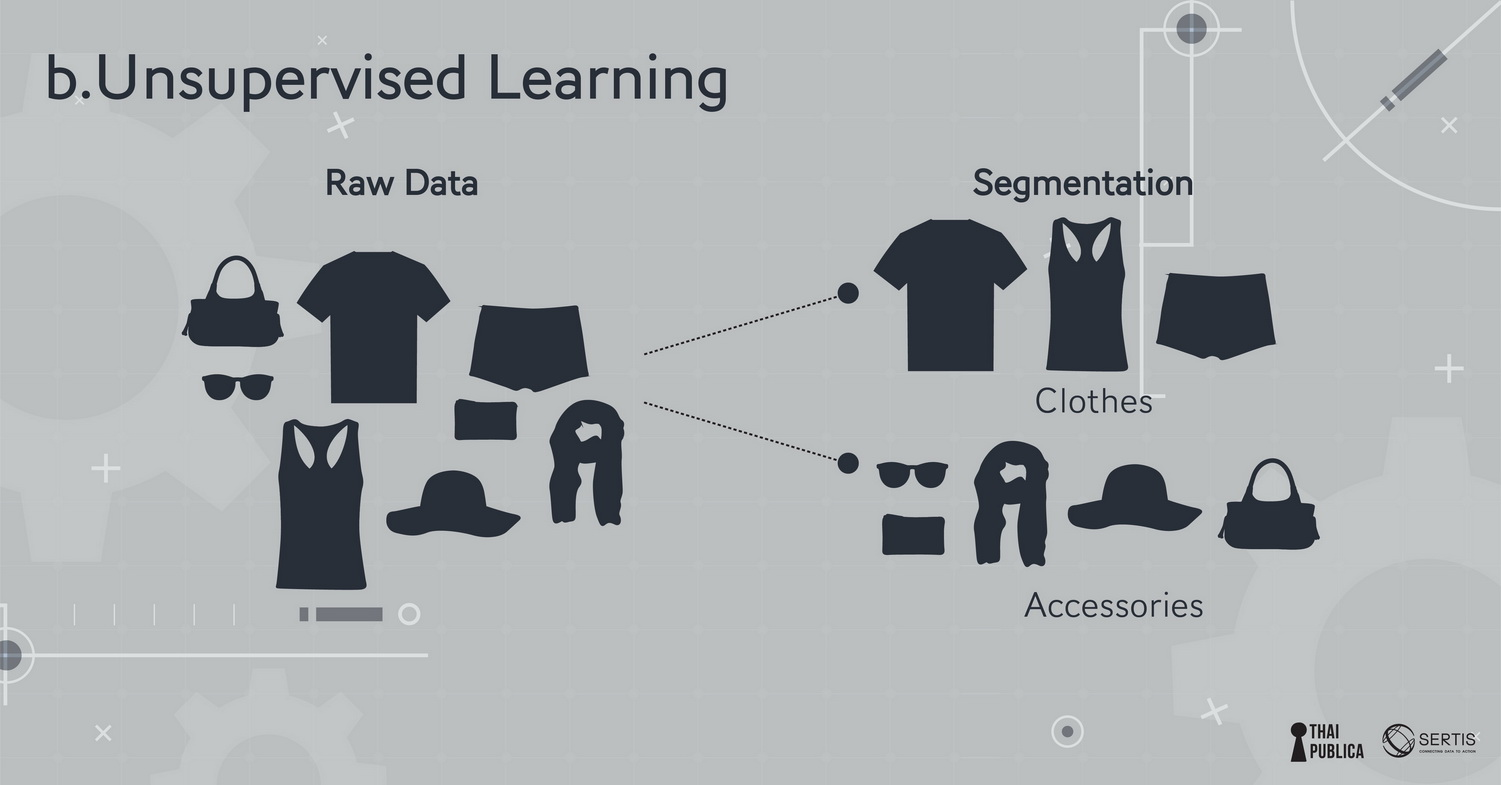
\includegraphics[width=0.8\textwidth]{Figures/2/8.jpg}
	% 				\caption{โมเดลที่ถูกสอนแบบ unsupervised learning}{ที่มา : https://thaipublica.org/2017/07/data-driven-society12/}
	% 				\label{Fig:Studentloan1}
	% 			\end{figure}
	% 		\end{itemize}


% 			\section{ความรู้พื้นฐานเกี่ยวกับการเรียนรู้ของเครื่อง (Machine Learning) }
% 			Firebase  \cite{vuejs} คือ Platform ที่รวบรวมเครื่องมือต่าง ๆ สำหรับการจัดการในส่วนของ Backend หรือ Server side ซึ่งทำให้สามารถ Build Mobile Application ได้อย่างมีประสิทธิภาพ และยังลดเวลาและค่าใช้จ่ายของการทำ Server side หรือการวิเคราะห์ข้อมูล โดยมีทั้งเครื่องมือที่ฟรี และเครื่องมีที่มีค่าใช้จ่าย 
% เครื่องมือ Firebase มีดังนี้
% 			\begin{enumerate}
% 				\item  Cloud Firestore คือ เครื่องมือ Database ที่เป็นลักษณะเป็น NoSQL โดยนำข้อดีของ Realtime Database ของ Firebase มาพัฒนาต่อ
% 				\item  Authentication  คือ  เครื่องมือ  Authentication ซึ่งคลอบคลุมทั้ง email-password, phone ไปจนถึง facebook, twitter, github สำหรับการ Login 
% 				\item  Hosting คือ hosting สำหรับ single-page web app, landing page website ซึ่งจัดการการ Deploy  และมีการติดตั้ง SSL ให้กับในส่วน Custom Domain  
% 				\item  Crashlytics ช่วยจัดการ Issue ต่าง ๆ และสามารถตรวจจับ Crash ได้ว่าเกิดขึ้นที่การทำงานไหนใน Mobile App 
% 				\item  Performance Monitoring  โดยผู้พัฒนาสามารถดู Performance ของ Code และ Network
% 			\end{enumerate}
			
\section{ความรู้พื้นฐานเกี่ยวกับการเรียนรู้เชิงลึก (Deep Learning)}
การเรียนรู้เชิงลึก \cite{deeplearning} คือโครงข่ายใยประสาทเสมือน (ANN: Artificial Neuron Networks) โดยการเรียนรู้เชิงลึกและโครงข่ายใยประสาทเสมือนเป็นอัลกอริทึมที่ถูกสร้างขึ้นมาเพื่อการเรียนรู้ของเครื่อง แต่ความแตกต่างระหว่างการเรียนรู้เชิงลึกกับโครงข่ายใยประสาทเสมือนคือชั้นซ่อนตัวที่ในการเรียนรู้เชิงลึกมีชั้นซ่อนตัวมากกว่าในโครงข่ายใยประสาทเสมือนโดยโครงข่ายใยประสาทเสมือนนั้นอาศัยแนวคิดและเทคนิคจากการทำงานของระบบโครงข่ายใยประสาทในระบบประสาทของมนุษย์ โดยจำลองการทำงานเหมือนกับกลุ่มเซลล์ประสาทที่เชื่อมโยงกันเป็นระบบประสาทที่สามารถรับรู้ได้หลายสิ่งในเวลาเดียวกัน ด้วยการประมวลผลแบบขนาน (Parallel Network) ทำให้ระบบสามารถตัดสินใจได้ใกล้เคียงกับมนุษย์ ในการที่เครื่องจะสามารถเข้าใจสิ่งอื่นได้ก็จำเป็นที่จะต้องมีองค์ความรู้ (Knowledge) เสียก่อนจากนั้นก็จะประเมินชุดข้อมูลและนำเสนอหรือแทนองค์ความรู้นั้น โดยมีกระบวนการทำงานดังรูปที่ \ref{fig:deep learning}

การเรียนรู้เชิงลึกถูกนำมาประยุกต์ใช้ในการทำงานเช่น การแยกแยะใบหน้าแต่ละคน ตัวอย่างเช่นในการติดแท็กรูปภาพเพื่อนใน Facebook หรือการแยกวัตถุที่ไม่ใช่คน หรือใช้เป็นส่วนหนึ่งในระบบรถยนต์ไร้คนขับ เป็นต้น
\begin{figure}[H]
	\centering
	\fbox{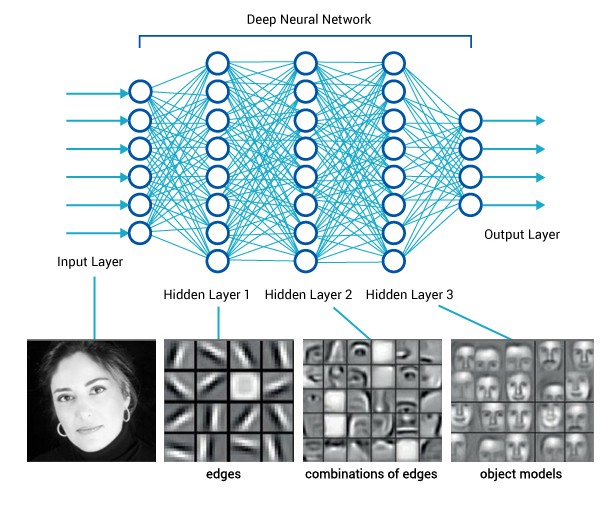
\includegraphics[scale=0.5]{Figures/2/deeplearning.jpeg}}
	\caption{ตัวอย่างการทำงานของการเรียนรู้เชิงลึก}{ที่มา: https://catalystsecure.com/blog/2017/07/deep-learning-in-e-discovery-moving-past-the-hype/}
	\label{fig:deep learning}
\end{figure}
\newpage
\section{ความรู้พื้นฐานเกี่ยวกับการเรียนรู้ของเครื่อง (Machine Learning)}
การเรียนรู้ของเครื่อง \cite{machinelearning} คือการทำให้คอมพิวเตอร์สามารถเรียนรู้ได้ด้วยตัวเองจากข้อมูลที่มีอยู่ ถ้าให้เปรียบเทียบแบบเห็นภาพชัดเจนคือเราเป็นครู คอมพิวเตอร์เป็นนักเรียนและความรู้เป็นข้อมูล แต่เดิมเราอยากสอนอะไรนักเรียน เราก็กางหนังสือแล้วถ่ายทอดความรู้ให้กับเด็ก ๆ ซึ่งนักเรียนก็จะเข้าใจความรู้นั้นเป็นก้อน แต่การเรียนรู้ของเครื่องคือการทำให้นักเรียนสามารถใช้ความรู้ (ข้อมูลที่ตัวเองมี) ในการวิเคราะห์ เชื่อมโยง คาดการณ์และประมวลผลได้ด้วยตัวเอง โดยไม่ต้องรอให้เราสอน

การเรียนรู้ของเครื่องมีรูปแบบการเรียนรู้ 3 รูปแบบ ดังนี้
\begin{itemize}[label={--}]
	\item การเรียนรู้แบบได้รับคำแนะนำ (Supervised learning)
	      เวลาป้อนข้อมูลให้กับคอมพิวเตอร์ (Input) เช่น รูปเสือ แต่คอมพิวเตอร์มันยังไม่รู้ว่าเป็นรูปเสือ เราก็ต้องบอกมันก่อน แล้วคอมพิวเตอร์ก็จะไปวิเคราะห์ (Feature Extraction) ว่า เสือเป็นสัตว์ 4 ขา มี 2 หู 1 หาง เป็นต้น จากนั้นคอมพิวเตอร์ก็นำข้อมูลดังกล่าวไปประมวลผล/จัดหมวดหมู่ (Classification) เพื่อให้หลังจากนี้มันสามารถแยกออกได้ว่าอะไรคือเสือ อะไรไม่ใช่เสือ
	
				\begin{figure}[H]
					\fbox{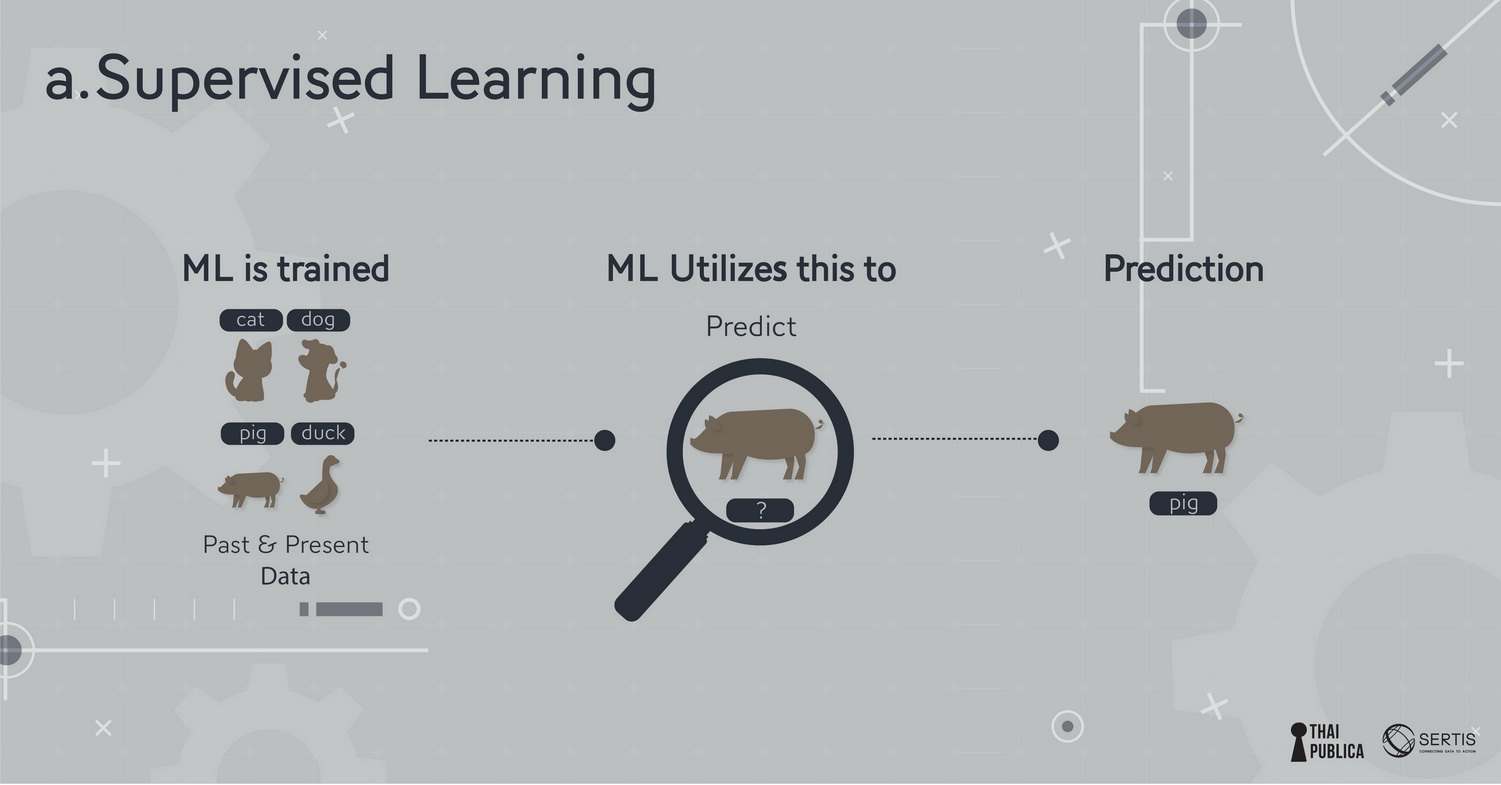
\includegraphics[width=\columnwidth]{Figures/2/7.jpg}}
					\caption{โมเดลที่ถูกสอนแบบ supervised learning}{ที่มา: https://thaipublica.org/2017/07/data-driven-society12/}
					\label{Fig:neural}
				\end{figure}
	
\item การเรียนรู้แบบไม่ได้รับคำแนะนำ (Unsupervised learning)
	      รูปแบบนี้เรียกได้ว่าตรงกันข้ามกับรูปแบบแรก มันคือการที่เราป้อนข้อมูล (Input) รูปเสือเข้าไป แต่ไม่ได้บอกมันว่ารูปที่ป้อนเข้าไปเป็นรูปเสือ เมื่อคอมพิวเตอร์มันเอาไปวิเคราะห์ (Feature Extraction) มันก็วิเคราะห์ได้นะว่ารูปที่ใส่เข้าไปมีลักษณะยังไง แต่คราวนี้มันไม่สามารถเอาไปประมวล/จัดหมวดหมู่ (Classification) ได้แล้ว มันจะใช้วิธีการแบ่งกลุ่มแทน (Clustering) ซึ่งคอมพิวเตอร์มันก็จะเอารูปเสือไปอยู่กับแมว สุนัข หรือสัตว์อื่น ๆ ที่มี 4 ขา มี 2 หู 1 หาง เหมือนกัน
				\begin{figure}[H]
					\fbox{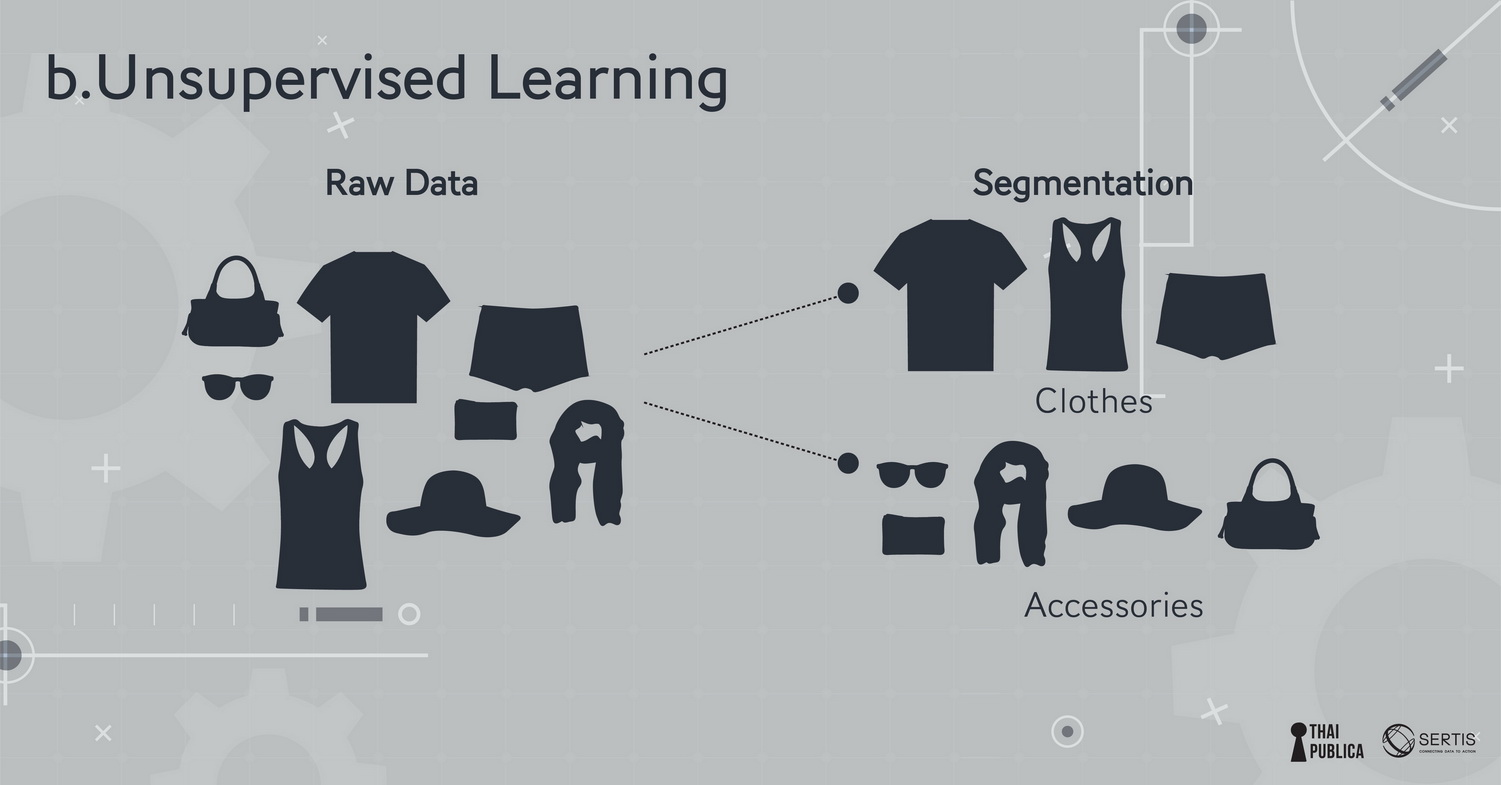
\includegraphics[width=\columnwidth]{Figures/2/8.jpg}}
					\caption{โมเดลที่ถูกสอนแบบ unsupervised learning}{ที่มา: https://thaipublica.org/2017/07/data-driven-society12/}
					\label{Fig:neural}
				\end{figure}
		\item การเรียนรู้แปบเสริมกำลัง (Reinforcement learning)
	      สามารถอธิบายได้ว่า เป็นการที่เรากำหนดเงื่อนไขบางอย่างให้กับคอมพิวเตอร์ แล้วทำให้คอมพิวเตอร์เอาชนะหรือทำตามเงื่อนไขนั้นให้ได้ ยกตัวอย่างเช่น Alpha Go เงื่อนไขของการเล่นหมากล้อมคือ ใช้หมากของตนล้อมพื้นที่บนกระดาน เพื่อให้ได้ดินแดนมากกว่าคู่ต่อสู้ ทีนี้ Alpha Go ก็จะเรียนรู้ด้วยตัวมันเองผ่านการจำลองการแข่งขันเป็นแสน ๆ ล้าน ๆ รอบ เพื่อให้รู้ว่า ถ้าหากคู่ต่อสู้เดินหมากนี้ ตัวมันเองจะเดินหมากไหนเพื่อให้บรรลุเงื่อนไขที่กำหนดไว้ให้ นั่นคือการยึดพื้นที่บนกระดานให้ได้มากที่สุด
				\begin{figure}[H]
					\fbox{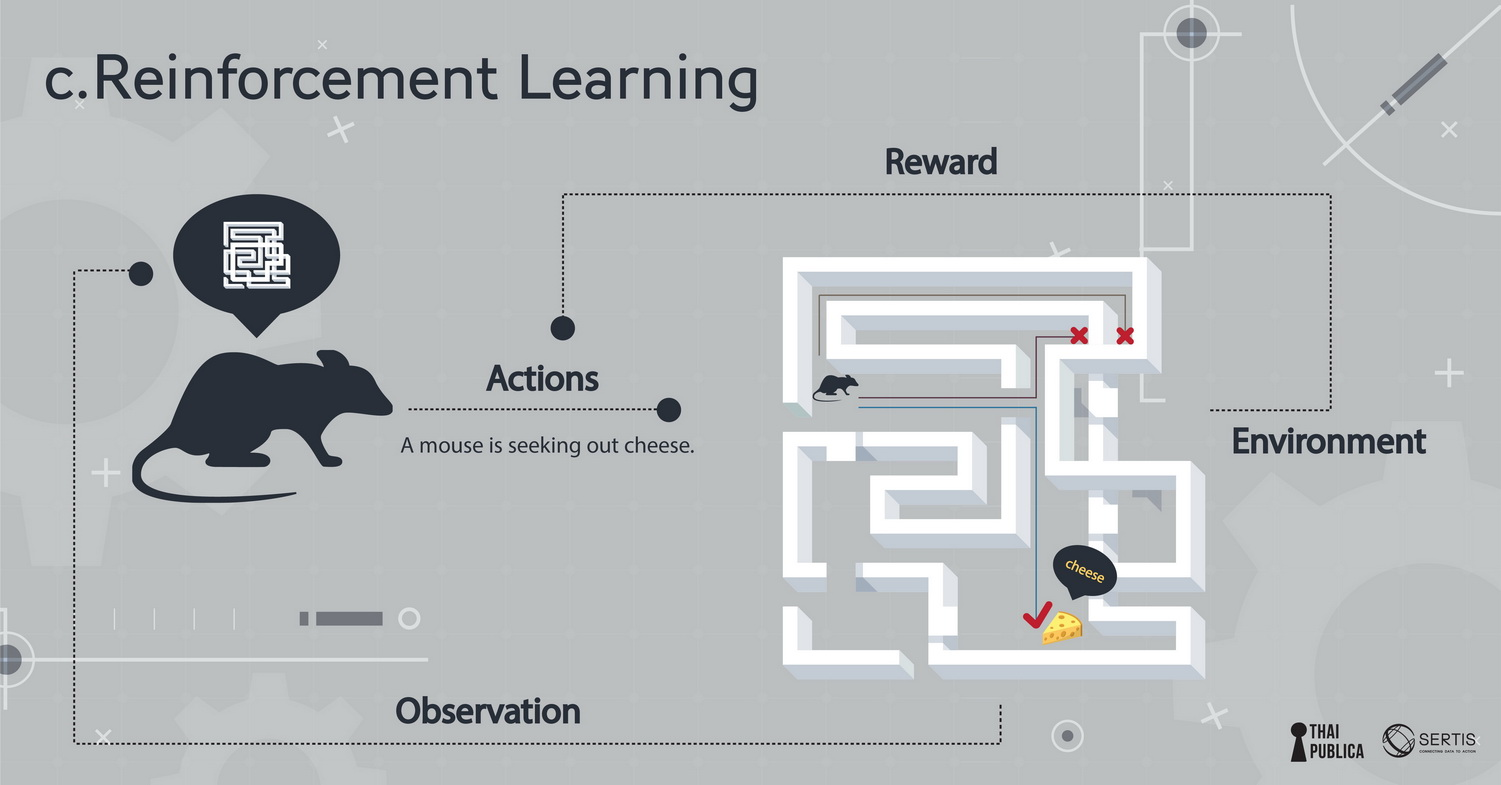
\includegraphics[width=\columnwidth]{Figures/2/un.jpg}}
					\caption{โมเดลที่ถูกสอนแบบ Reinforcement learning}{ที่มา: https://thaipublica.org/2017/07/data-driven-society12/}
					\label{Fig:neural}
				\end{figure}
			\end{itemize}

\section{ความรู้พื้นฐานเกี่ยวกับโครงข่ายประสาทเทียม (Neural Network)}
โครงข่ายประสาทเทียมคือโครงข่ายประสามเทียมที่เป็นการจำลองมาจากสมองของมนุษย์ โดยสมองของเรานั้นจะมีหน่วยประมวลผลขนาดเล็กอยู่เป็นจำนวนมาก และเชื่อมโยงกันด้วยโครงข่ายประสาท ช่วยให้มนุษย์สามารถเรียนรู้และคิดวิเคราะห์ได้อย่างรวดเร็ว แต่ในส่วนคอมพิวเตอร์นั้นไม่ได้มีโครงข่ายที่ซับซ้อนเหมือนกับสมองของมนุษย์ มันมีหน้าที่เพียงรันโปรแกรมตามคำสั่งของมนุษย์เท่านั้น ดังนั้นเมื่อต้องการให้มันทำการเรียนรู้บางอย่าง จึงเป็นเรื่องยากในรูปแบบปกติ จึงเกิดการจำลองแนวทางการเรียนรู้ของมนุษย์ไปสู่คอมพิวเตอร์ด้วยโครงข่ายประสาทเทียม \cite{neural}

โดยส่วนที่เล็กที่สุดของโครงข่ายประสาทเทียมคือ Neuron ทำหน้าที่คำนวนข้อมูลรับเข้าเพื่อให้ได้ผลลัพธ์ออกไป โดยในรูปที่ \ref{Fig:neural} มีส่วนประกอบสำคัญดังนี้
\begin{itemize}[label={--}]
	\item Input หรือค่าที่ส่งเข้ามาที่ Neuron โดยจะมีขาที่เข้ามาได้หลายขา ขึ้นอยู่กับเราจะสร้าง
	\item Weight เป็นการให้น้ำหนักของขาแต่ละที่ส่งเข้ามา โดยมีค่าระหว่าง 0-1 เมื่อเริ่มต้นจะเป็นการ Random ขึ้นมา จากนั้นตัว Neuron เมื่อทำการเรียนรู้จะเป็นการปรับ weight ตัวเอง เพื่อให้มันได้คำตอบที่ใกล้เคียงที่สุด
	\item Bias คือค่าที่จะช่วยเข้ามาทำให้ค่าที่เข้ามาอยู่ในระหว่าง 0 - 1 ได้ โดยจะเป็นเลข random และปรับทุกครั้งที่เรียนรู้
	\item Output คือผลลัพธ์
	\item Back Propagation คือการที่ Neuron นำค่า Error ของ Output ที่ได้ กับ Output ที่เราสั่งให้มันเรียนรู้ นำไปปรับ Weight และ Bias ให้เกิดผลลัพธ์ที่ถูกต้องตามที่ได้เรียนรู้มา
\end{itemize}
\begin{figure}[H]
	\fbox{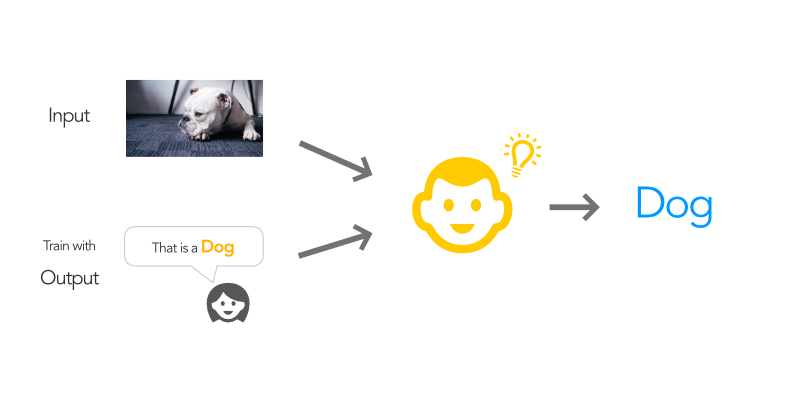
\includegraphics[width=\columnwidth]{Figures/2/neural.png}}
	\caption{ตัวอย่างของโครงข่ายประสาท}{ที่มา: https://coladev.com/machine-learning/neural-network/2017/02/22/neural-network-basic}
	\label{Fig:neural}
\end{figure}




	\section{ความรู้พื้นฐาน Firebase }
				Firebase  \cite{fi} คือ Platform ที่รวบรวมเครื่องมือต่าง ๆ สำหรับการจัดการในส่วนของ Backend หรือ Server side ซึ่งทำให้สามารถ Build Mobile Application ได้อย่างมีประสิทธิภาพ และยังลดเวลาและค่าใช้จ่ายของการทำ Server side หรือการวิเคราะห์ข้อมูล โดยมีทั้งเครื่องมือที่ฟรี และเครื่องมีที่มีค่าใช้จ่าย \cite{fi}
เครื่องมือ Firebase มีดังนี้
				\begin{enumerate}
					\item  Cloud Firestore คือ เครื่องมือ Database ที่เป็นลักษณะเป็น NoSQL โดยนำข้อดีของ Realtime Database ของ Firebase มาพัฒนาต่อ
					\item  Authentication  คือ  เครื่องมือ  Authentication ซึ่งคลอบคลุมทั้ง email-password, phone ไปจนถึง facebook, twitter, github สำหรับการ Login 
					\item  Hosting คือ hosting สำหรับ single-page web app, landing page website ซึ่งจัดการการ Deploy  และมีการติดตั้ง SSL ให้กับในส่วน Custom Domain  
					\item  Crashlytics ช่วยจัดการ Issue ต่าง ๆ และสามารถตรวจจับ Crash ได้ว่าเกิดขึ้นที่การทำงานไหนใน Mobile App 
					\item  Performance Monitoring  โดยผู้พัฒนาสามารถดู Performance ของ Code และ Network
				\end{enumerate}

						
			